\documentclass[11pt]{article}

\usepackage[utf8]{inputenc}
\usepackage[T1]{fontenc}

\usepackage{fullpage}

\usepackage{graphicx}
\usepackage{verbatim}
\usepackage{siunitx}
\usepackage{pgfplots}

\usepackage[colorlinks=false,pdfborder={0 0 0}]{hyperref}
\usepackage[all]{hypcap}


\title{Astro 585: HW 6}
\author{Codename: The Maxwell-Jüttner Distribution}



\begin{document}


\maketitle

My git repository is here: \url{https://github.com/hsgg/astro585}, clone URL
\url{https://github.com/hsgg/astro585.git}.


\section{Parallel stuff}

1a) nprocs() is one larger than nworkers(). So there seems to be one process
that manages all the ones that will do the actual computation.

1b) As you told us, the functions are only defined on the main process, not the
workers.

1c) Presumably every worker writes to their own copy of 'integral', and the
main thread doesn't do anything, so 'integral' in the main thread remains 0.0.

pmap(): Looks like the main process is using one thread (ca~95\%), the other
two share the other one, but they don't use as much (ca 40\% each).

map(): Uses only one processor at a time. That's strange. The distributed array
seems to make it really slow. Not distributing makes the operation finish in
much less than a second, rather than 10s.

OK, I am not yet convinced of distributed arrays, although it seems to make
sense. There is significant overhead involved with this.


\section{Kepler}

185~seconds when running in serial. Oddly, my plot looks differnt than yours
when running your code:
\begin{center}
	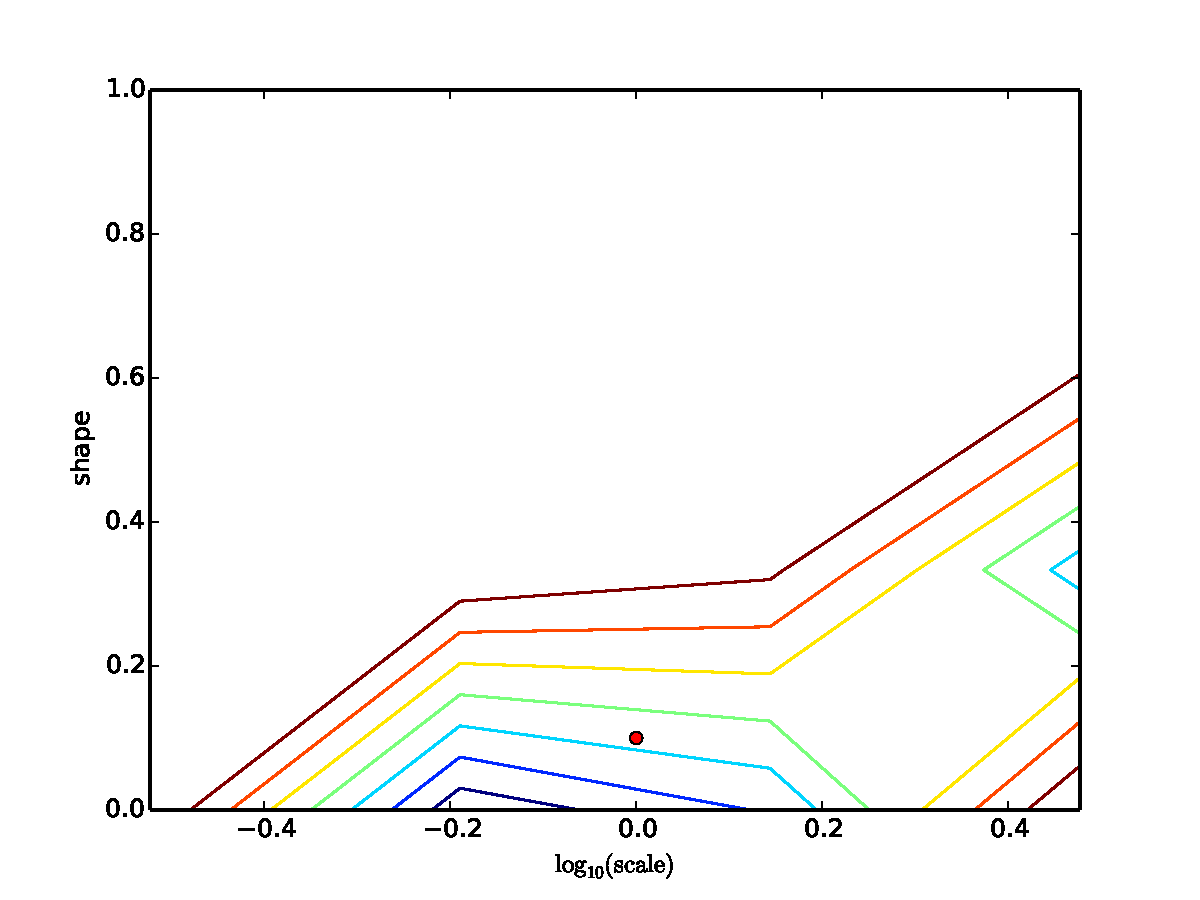
\includegraphics[width=0.7\textwidth]{parameterspace_originalserial.pdf}
\end{center}

101~seconds in parallel with 2 cores, so slightly more than half the time, with
almost the same result. There is a difference close to (0.0,~0.0). Not good:
\begin{center}
	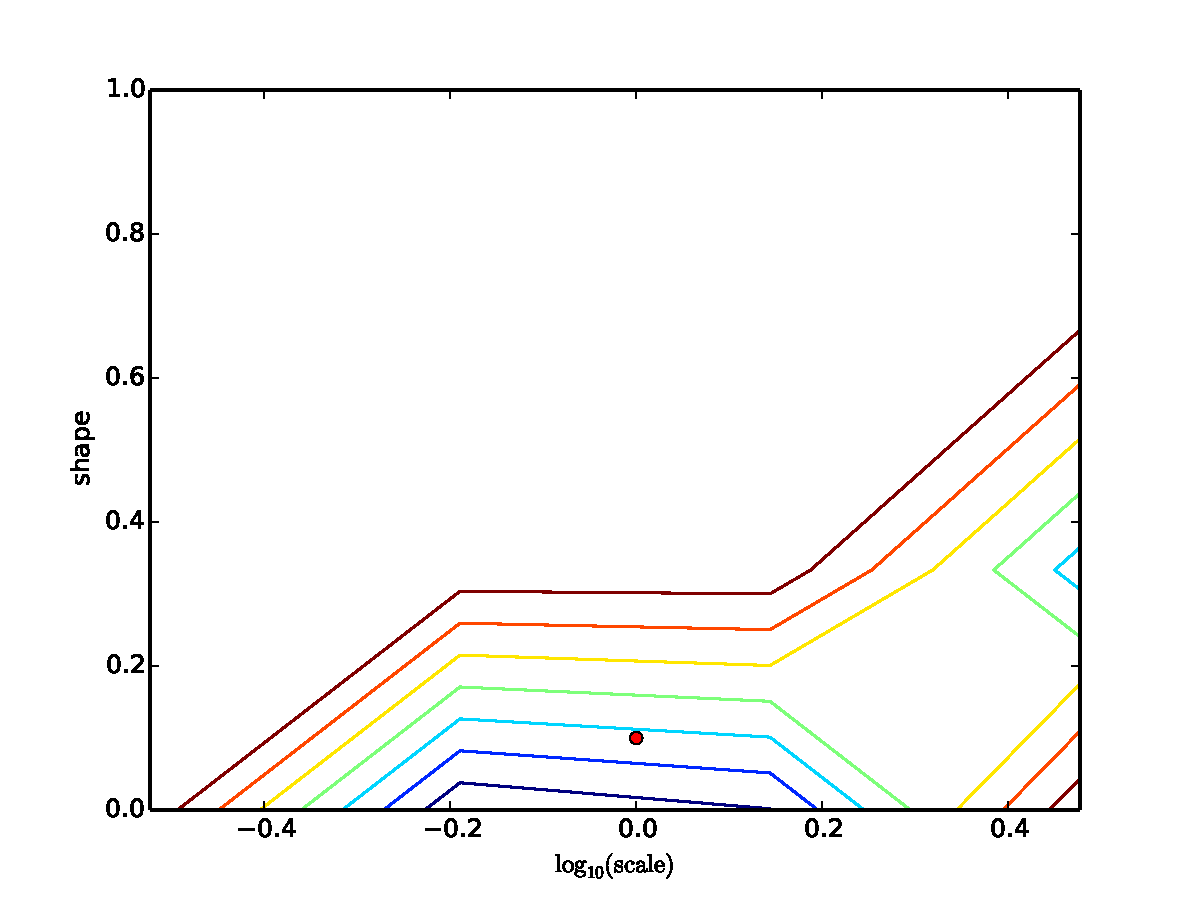
\includegraphics[width=0.7\textwidth]{parameterspace_parallel.pdf}
\end{center}

Using distributed arrays wouldn't change the performance much, because there is
little overhead due to communication. There are a total of 64 different points
in parameter space to test, or 192 floats, and the return value is also just a
list of 64 floats. Not much communication.

On workstation with 4 cores (yeah, I know, 4 != 8):
\begin{center}
  \begin{tikzpicture}[font=\Large]
    \begin{axis}[
        ymin=0,
        xlabel=Number of worker processes,
        ylabel=Computation time in wall-seconds
      ]
      \addplot coordinates {
        (0, 27.644736393)
        (1, 105.609920487)
        (2, 58.597616588)
        (3, 45.131695724)
        (4, 37.878587973)
        (5, 38.968469081)
        (6, 38.930108833)
        (7, 37.319774925)
        (8, 37.690685883)
      };
    \end{axis}
  \end{tikzpicture}
\end{center}
I am surprised by the fact that the single-threaded version is so much faster
than even using 4 worker threads. I would not expect much communication
overhead, since we are only transferring a few hundred floats from process to
process.

Turning 'parameterspace' into a distributed array did not have any effect,
either. I guess that is expected if there is not much data being communicated.

The code:
\verbatiminput{6.2_planets.jl}

\end{document}
